\documentclass[smallextended]{svjour3}
\usepackage[T1]{fontenc}
\usepackage[utf8]{inputenc}
\usepackage{mathptmx}
\usepackage{amsmath,graphicx,booktabs,tabularx,longtable,url,placeins}
\usepackage[hidelinks]{hyperref}
\journalname{Computing}
\setlength{\emergencystretch}{2em}
\renewcommand{\thefigure}{S\arabic{figure}}
\renewcommand{\thetable}{S\arabic{table}}
\begin{document}
\title{Online Resource 1: Evaluating Candidate-Restricted Influence Maximization: Effects of Reference Budget and Ranking Precision}
\titlerunning{Online Resource 1}
\author{Jiayue Sun \and Binbin Yong \and Junjie An \and Tianyu Bo \and Shuai Li}
\institute{Jiayue Sun \at School of Artificial Intelligence, Lanzhou University, Lanzhou 730000, China
\and Binbin Yong (corresponding author) \at School of Information Science and Engineering, Lanzhou University, Lanzhou 730000, China \\
\email{yongbb14@lzu.edu.cn}
\and Junjie An, Tianyu Bo and Shuai Li \at Lanzhou University, Lanzhou, China}
\date{}\maketitle
\paragraph{Scope.} External results and the 520-condition historical extension form separate evidence layers. The initial 42-condition study supplies earlier context; outcome-blind preflight supplies resource measurements only. Historical tables and figures report descriptive recomputations of saved outputs, separately from the external main experiments and post-hoc PageRank sensitivity controls.

\section{Source-scoped related-work comparison}
Table~\ref{tab:related-scope} compares the stated focus of accessible primary
sources, rather than asserting that an item was absent from every implementation
or supplement. ``Not the stated focus'' is not shorthand for ``not done''.
Classical objective/solver work, benchmarking, candidate restriction and learned
inductive estimation address different parts of the influence-maximization
pipeline. This study provides paired evidence on the precision dependence of a
budget comparison, the utility consequences of reference-set changes, and the
external scope of candidate-restriction results. Complete citations are in the
main manuscript.
\begin{table}[htbp]
\caption{Source-scoped comparison of stated evaluation focus. ``Not the stated focus'' does not assert that a feature was absent from every implementation or supplement.}\label{tab:related-scope}
\begin{tabularx}{\linewidth}{p{.19\linewidth}p{.31\linewidth}X}
\toprule
Study & Stated object and role of eligibility & Evaluation dimensions relevant here \\
\midrule
Kempe et al. (2003); CELF/IMM & Expected-spread objective and faster seed selection; fixed full eligibility in the standard formulation & Candidate restriction, held-out utility, cross-budget reference changes, ranking precision and coverage are not the stated comparative object. \\
StaticGreedy (2013) & Reused static realizations for scalable influence maximization & Fixed-world construction is central; this paper does not treat its solver result as evidence about the present restricted-pool evaluation chain. \\
Arora et al. (2017) & Comparative benchmarking of influence-maximization methods & Quality and running-time comparability are relevant; the stated benchmark focus differs from cross-budget evaluation of a fixed truncated ranking. \\
Rui et al. (2020) & Influence estimation from multiple neighbourhood levels & The publisher abstract describes influence scoring and seed selection; it does not establish a matched test of ranking tolerance and reference budget. \\
Ko et al. (2025) & Learned inductive influence estimation/maximization & It changes the estimator and evaluates held-out networks; this differs from preserving a simulator while diagnosing a fixed ranking truncation. \\
This study & Fixed candidate restrictions against finite-world full references & Reports coverage, budget, ranking tolerance, sequence/set agreement, spread estimated on independent evaluation worlds, coupling and scoped costs jointly. \\
\bottomrule
\end{tabularx}
\end{table}


\section{Audit and reproducibility}
Figures~\ref{fig:matrix}--\ref{fig:loss-cost} provide the full default-budget
comparison, the direction diagnostic and the descriptive loss--cost analysis,
complementing the main-text evaluation framework, budget--precision comparison
and independent reference-transition plot.

There are 54 configuration-defined external conditions and 468 executed arms.
The archive retains one JSON and NPZ pair per condition, source and data manifests,
world-ID hashes, candidate IDs, selected sequences, all round/candidate integer
totals and 10,000 evaluation values per arm. Reproduction checks the raw gzip
hashes before using the frozen runner. The independent audit
parses topology, checks all recorded hashes and world IDs, reconstructs all
argmax/tie decisions, replays every full-candidate score matrix and all evaluation
arrays, and checks a scalar Python oracle on the first 16 worlds for each
distinct ordered selection within a graph/path/coupling. Complete replay and the
independent sampled oracle are different validation layers.

Frozen source files are unchanged. The original runner's entry checks did not
enforce actual raw hashes against the data manifest; the retrospective comparison
and new guarded wrapper address that enforcement gap without rewriting history.
ca-GrQc removes loops before collecting endpoints: raw vertex 12295 appears only
in a loop, explaining 5,241 rather than 5,242 vertices. The original prose was
ambiguous about endpoint collection order, while the processed size/hash were
already frozen before outcomes. Results refer to that processed graph.

Direction is part of the simulation definition. CollegeMsg goes from sender to
receiver; wiki-Vote from voter to votee; ca-GrQc uses reciprocal arcs. The first
two are directed observed relations, not measured causal diffusion. PageRank uses
standard incoming importance, while the objective follows outgoing propagation.
Direction diagnostics are post-hoc and do not isolate a causal mechanism.

\subsection{Preprocessing and evidence provenance}
CollegeMsg retains the first $\lfloor .65T\rfloor$ complete timestamp groups,
where $T=58,911$, through Unix timestamp 1085640224, yielding 38,939 non-self
messages. The processed CollegeMsg, ca-GrQc and wiki-Vote graphs have 2, 354 and
24 weak components. Every retained component is included. The later CollegeMsg
events are not held-out influence cascades. The ca-GrQc size and hash were
recorded before outcomes; reinserting its self-loop-only vertex would change
lexical indices and hashed draws, so the 5,241-node representation defines the
reported experiment.

The initial historical study contains 42 conditions and 168 arms, two paths,
$W=20,80,320$ and $M=2000$. Its separate extension contains 520 conditions and
4,680 arms, ten paths on four real contact graphs, selection budgets up to 5120
and $M=10,000$. The four contact graphs contain 91, 212, 402 and 75 vertices;
two synthetic controls contain 2,000 vertices each. Synthetic topology weights
are not independent historical-event evidence. Local protocol freezes are not
public preregistrations. External resource preflight used $W=80,320$ and
$M=1000$ without examining selected seeds or utilities; it supplies resource
measurements only.

\subsection{Finite-world coupling counterexample}
Consider the chain $s\to u\to v$ with horizon two. In one step-indexed world,
$s\to u$ is open at step zero, while $u\to v$ is closed at step zero and open
at step one. Starting with $\{s\}$ reaches all three vertices. Starting with
$\{s,u\}$ activates $u$ earlier and reaches only two. Thus the finite-world
objective is not necessarily monotone, even though the marginal law for each
fixed seed set remains the intended independent-cascade law. This example alone
does not establish a violation of submodularity. The fixed-edge control instead
uses horizon-limited reachability in each sampled graph, giving a monotone,
submodular coverage objective. Both implementations enumerate all eligible
vertices at every round. The external world-ID audit checks 169,200 distinct
identifiers across graph, path and selection/evaluation families for collisions.

\section{Statistical interpretation}
For a fixed selected pair, conditional Monte Carlo standard error is the sample
standard deviation of 10,000 paired per-world differences divided by 100.
Normal intervals are pointwise and conditional. Across-path SD describes five
computational paths, or three control paths, and includes finite evaluation noise.
The optional $t$ intervals in CSVs are post-hoc descriptive intervals, not
population-of-network inference. Random pools are averaged within each path
before cross-path analysis; their shared-world covariance is retained.

For a seed set of size $k$, incremental spread is total spread minus $k$.
The external experiments use $k=5$; the historical extension also includes $k=20$.
Percentage loss is
minus the paired mean difference divided by full incremental spread, times 100.
The plug-in percentage does not have a guaranteed loss-bound interpretation.
The primary sign-test family is three methods within each graph at $W=1280$.
All nonzero PageRank and random-mean differences are negative, but five paths
limit the minimum two-sided exact sign-test value to .0625. Nonsignificance is
not equivalence. Table~\ref{tab:tests} reports all nine tests without exclusions.

\section{Cost and repeated measurements}
The archived preparation timer contains parsing, all rankings, hashes and graph
diagnostics. Its ranking subtimers are not added to it again. A separate
post-hoc setup study measures five repetitions of raw parsing/CSR and one
method's ranking plus pool generation. The frozen selection timer already includes
lexical candidate sorting; it is not charged again. The assembled selection-use cost adds that
median setup to frozen selection-world preparation and selection. The assembled cost including independent evaluation adds independent-world preparation and independent evaluation.
These are assembled warm-process, cached-file estimates, not direct end-to-end
trials. Imports, JIT compilation, downloads and output writing are excluded.

Frozen repeated timing uses path 1101 and $W=320$, five randomized repetitions
per arm, yielding 130 observations. Selected sequences and per-world evaluations
were required to remain identical. The CSVs report every repetition and its
selection/evaluation time, plus medians and ranges. The maximum positive psutil process-lifetime peak is 3.448822 GiB. Preflight
used one tenth of the evaluation-world count and therefore has a different
resource scope; the recorded peak is not a condition-specific allocation maximum. Timings are machine- and implementation-specific.

\section{Complete aggregate results}
Tables~\ref{tab:s-ca_grqc}--\ref{tab:s-wiki_vote} retain every method at all external
budgets/couplings. Total spread, paired difference, between-path SD, percentage
incremental loss and ordered agreement are shown. CSVs additionally retain
candidate fractions, set agreement, Jaccard, first divergence, conditional
uncertainty, costs and every path. This avoids treating an averaged random seed
set as if it existed. There were no failed or excluded main conditions.
\begin{table}[htbp]
\caption{Prespecified primary exact two-sided sign tests at $W=1280$. Holm correction is across three methods within each fixed graph. Zero path differences are dropped from the sign test.}\label{tab:tests}
\begin{tabular}{llrrrr}
\toprule
Graph & Method & Mean $\Delta$ & Zeros & $p$ & Holm $p$ \\
\midrule
CollegeMsg & Degree-4k & 0.00000 & 5 & 1.0000 & 1.0000 \\
CollegeMsg & PageRank-4k & -0.90780 & 0 & 0.0625 & 0.1875 \\
CollegeMsg & Random mean & -8.22745 & 0 & 0.0625 & 0.1875 \\
ca-GrQc & Degree-4k & 0.00000 & 5 & 1.0000 & 1.0000 \\
ca-GrQc & PageRank-4k & -0.25082 & 0 & 0.0625 & 0.1875 \\
ca-GrQc & Random mean & -3.94366 & 0 & 0.0625 & 0.1875 \\
wiki-Vote & Degree-4k & 0.00000 & 5 & 1.0000 & 1.0000 \\
wiki-Vote & PageRank-4k & -40.69334 & 0 & 0.0625 & 0.1875 \\
wiki-Vote & Random mean & -50.90179 & 0 & 0.0625 & 0.1875 \\
\bottomrule
\end{tabular}
\end{table}

\begin{table}[htbp]
\caption{ca-GrQc: complete frozen aggregate matrix; PageRank uses default tolerance. E means fixed-edge coupling (three paths); other rows use five step-coupled paths. Total is total spread (nodes); $\Delta$ is restricted minus full spread (nodes); SD is across path mean differences. Random pools are averaged within each path; their agreement entry is a fraction.}\label{tab:s-ca_grqc}
\begin{tabular}{rlrrrrr}
\toprule
$W$ & Method & Total & $\Delta$ & SD & Loss (\%) & Order \\
\midrule
80 & Degree-4k & 9.636 & +0.226 & 0.190 & -5.16 & 1/5 \\
80 & Degree-5\% & 9.410 & +0.000 & 0.000 & 0.00 & 5/5 \\
80 & Full & 9.410 & +0.000 & 0.000 & 0.00 & 5/5 \\
80 & PageRank-4k & 9.646 & +0.236 & 0.274 & -5.61 & 0/5 \\
80 & PageRank-5\% & 9.522 & +0.111 & 0.125 & -2.62 & 2/5 \\
80 & Random mean & 5.961 & -3.449 & 0.303 & 78.14 & 0.00 \\
320 & Degree-4k & 9.845 & +0.038 & 0.086 & -0.83 & 4/5 \\
320 & Degree-5\% & 9.806 & +0.000 & 0.000 & 0.00 & 5/5 \\
320 & Full & 9.806 & +0.000 & 0.000 & 0.00 & 5/5 \\
320 & PageRank-4k & 9.680 & -0.126 & 0.181 & 2.53 & 0/5 \\
320 & PageRank-5\% & 9.806 & +0.000 & 0.000 & 0.00 & 5/5 \\
320 & Random mean & 5.983 & -3.824 & 0.272 & 79.50 & 0.00 \\
1280 & Degree-4k & 9.934 & +0.000 & 0.000 & 0.00 & 5/5 \\
1280 & Degree-5\% & 9.934 & +0.000 & 0.000 & 0.00 & 5/5 \\
1280 & Full & 9.934 & +0.000 & 0.000 & 0.00 & 5/5 \\
1280 & PageRank-4k & 9.683 & -0.251 & 0.076 & 5.07 & 0/5 \\
1280 & PageRank-5\% & 9.934 & +0.000 & 0.000 & 0.00 & 5/5 \\
1280 & Random mean & 5.990 & -3.944 & 0.221 & 79.90 & 0.00 \\
320E & Degree-4k & 9.934 & +0.082 & 0.079 & -1.70 & 1/3 \\
320E & Degree-5\% & 9.852 & +0.000 & 0.000 & 0.00 & 3/3 \\
320E & Full & 9.852 & +0.000 & 0.000 & 0.00 & 3/3 \\
320E & PageRank-4k & 9.689 & -0.162 & 0.086 & 3.33 & 0/3 \\
320E & PageRank-5\% & 9.904 & +0.052 & 0.090 & -1.09 & 2/3 \\
320E & Random mean & 6.108 & -3.744 & 0.137 & 77.16 & 0.00 \\
\bottomrule
\end{tabular}
\end{table}

\begin{table}[htbp]
\caption{CollegeMsg: complete frozen aggregate matrix; PageRank uses default tolerance. E means fixed-edge coupling (three paths); other rows use five step-coupled paths. Total is total spread (nodes); $\Delta$ is restricted minus full spread (nodes); SD is across path mean differences. Random pools are averaged within each path; their agreement entry is a fraction.}\label{tab:s-college_msg}
\begin{tabular}{rlrrrrr}
\toprule
$W$ & Method & Total & $\Delta$ & SD & Loss (\%) & Order \\
\midrule
80 & Degree-4k & 14.919 & +0.000 & 0.000 & 0.00 & 5/5 \\
80 & Degree-5\% & 14.919 & +0.000 & 0.000 & 0.00 & 5/5 \\
80 & Full & 14.919 & +0.000 & 0.000 & 0.00 & 5/5 \\
80 & Weighted-4k & 14.597 & -0.322 & 0.229 & 3.21 & 0/5 \\
80 & Weighted-5\% & 14.919 & +0.000 & 0.000 & 0.00 & 5/5 \\
80 & PageRank-4k & 13.991 & -0.928 & 0.295 & 9.33 & 0/5 \\
80 & PageRank-5\% & 14.461 & -0.457 & 0.297 & 4.57 & 0/5 \\
80 & Random mean & 6.804 & -8.114 & 0.146 & 81.84 & 0.00 \\
320 & Degree-4k & 15.019 & +0.000 & 0.000 & 0.00 & 5/5 \\
320 & Degree-5\% & 15.019 & +0.000 & 0.000 & 0.00 & 5/5 \\
320 & Full & 15.019 & +0.000 & 0.000 & 0.00 & 5/5 \\
320 & Weighted-4k & 14.820 & -0.199 & 0.130 & 1.97 & 0/5 \\
320 & Weighted-5\% & 15.019 & +0.000 & 0.000 & 0.00 & 5/5 \\
320 & PageRank-4k & 14.164 & -0.854 & 0.117 & 8.52 & 0/5 \\
320 & PageRank-5\% & 14.645 & -0.374 & 0.125 & 3.72 & 0/5 \\
320 & Random mean & 6.836 & -8.183 & 0.211 & 81.70 & 0.00 \\
1280 & Degree-4k & 15.072 & +0.000 & 0.000 & 0.00 & 5/5 \\
1280 & Degree-5\% & 15.072 & +0.000 & 0.000 & 0.00 & 5/5 \\
1280 & Full & 15.072 & +0.000 & 0.000 & 0.00 & 5/5 \\
1280 & Weighted-4k & 14.820 & -0.252 & 0.024 & 2.50 & 0/5 \\
1280 & Weighted-5\% & 15.072 & +0.000 & 0.000 & 0.00 & 5/5 \\
1280 & PageRank-4k & 14.164 & -0.908 & 0.041 & 9.01 & 0/5 \\
1280 & PageRank-5\% & 14.641 & -0.431 & 0.043 & 4.28 & 0/5 \\
1280 & Random mean & 6.845 & -8.227 & 0.266 & 81.69 & 0.00 \\
320E & Degree-4k & 15.062 & +0.000 & 0.000 & 0.00 & 3/3 \\
320E & Degree-5\% & 15.062 & +0.000 & 0.000 & 0.00 & 3/3 \\
320E & Full & 15.062 & +0.000 & 0.000 & 0.00 & 3/3 \\
320E & Weighted-4k & 14.790 & -0.272 & 0.037 & 2.71 & 0/3 \\
320E & Weighted-5\% & 15.062 & +0.000 & 0.000 & 0.00 & 3/3 \\
320E & PageRank-4k & 14.128 & -0.934 & 0.031 & 9.28 & 0/3 \\
320E & PageRank-5\% & 14.631 & -0.431 & 0.046 & 4.28 & 0/3 \\
320E & Random mean & 6.925 & -8.137 & 0.293 & 80.87 & 0.00 \\
\bottomrule
\end{tabular}
\end{table}

\begin{table}[htbp]
\caption{wiki-Vote: complete frozen aggregate matrix; PageRank uses default tolerance. E means fixed-edge coupling (three paths); other rows use five step-coupled paths. Total is total spread (nodes); $\Delta$ is restricted minus full spread (nodes); SD is across path mean differences. Random pools are averaged within each path; their agreement entry is a fraction.}\label{tab:s-wiki_vote}
\begin{tabular}{rlrrrrr}
\toprule
$W$ & Method & Total & $\Delta$ & SD & Loss (\%) & Order \\
\midrule
80 & Degree-4k & 60.736 & +0.000 & 0.000 & 0.00 & 5/5 \\
80 & Degree-5\% & 60.736 & +0.000 & 0.000 & 0.00 & 5/5 \\
80 & Full & 60.736 & +0.000 & 0.000 & 0.00 & 5/5 \\
80 & PageRank-4k & 20.043 & -40.693 & 0.138 & 73.01 & 0/5 \\
80 & PageRank-5\% & 46.855 & -13.882 & 0.107 & 24.91 & 0/5 \\
80 & Random mean & 9.775 & -50.961 & 1.921 & 91.43 & 0.00 \\
320 & Degree-4k & 60.736 & +0.000 & 0.000 & 0.00 & 5/5 \\
320 & Degree-5\% & 60.736 & +0.000 & 0.000 & 0.00 & 5/5 \\
320 & Full & 60.736 & +0.000 & 0.000 & 0.00 & 5/5 \\
320 & PageRank-4k & 20.014 & -40.722 & 0.112 & 73.06 & 0/5 \\
320 & PageRank-5\% & 46.986 & -13.750 & 0.250 & 24.67 & 0/5 \\
320 & Random mean & 9.831 & -50.905 & 1.897 & 91.33 & 0.00 \\
1280 & Degree-4k & 60.736 & +0.000 & 0.000 & 0.00 & 5/5 \\
1280 & Degree-5\% & 60.736 & +0.000 & 0.000 & 0.00 & 5/5 \\
1280 & Full & 60.736 & +0.000 & 0.000 & 0.00 & 5/5 \\
1280 & PageRank-4k & 20.043 & -40.693 & 0.138 & 73.01 & 0/5 \\
1280 & PageRank-5\% & 47.206 & -13.530 & 0.096 & 24.28 & 0/5 \\
1280 & Random mean & 9.834 & -50.902 & 1.892 & 91.33 & 0.00 \\
320E & Degree-4k & 60.663 & +0.000 & 0.000 & 0.00 & 3/3 \\
320E & Degree-5\% & 60.663 & +0.000 & 0.000 & 0.00 & 3/3 \\
320E & Full & 60.663 & +0.000 & 0.000 & 0.00 & 3/3 \\
320E & PageRank-4k & 20.087 & -40.576 & 0.003 & 72.90 & 0/3 \\
320E & PageRank-5\% & 47.050 & -13.613 & 0.209 & 24.46 & 0/3 \\
320E & Random mean & 9.394 & -51.269 & 1.963 & 92.11 & 0.00 \\
\bottomrule
\end{tabular}
\end{table}

\begin{figure}[htbp]
\centering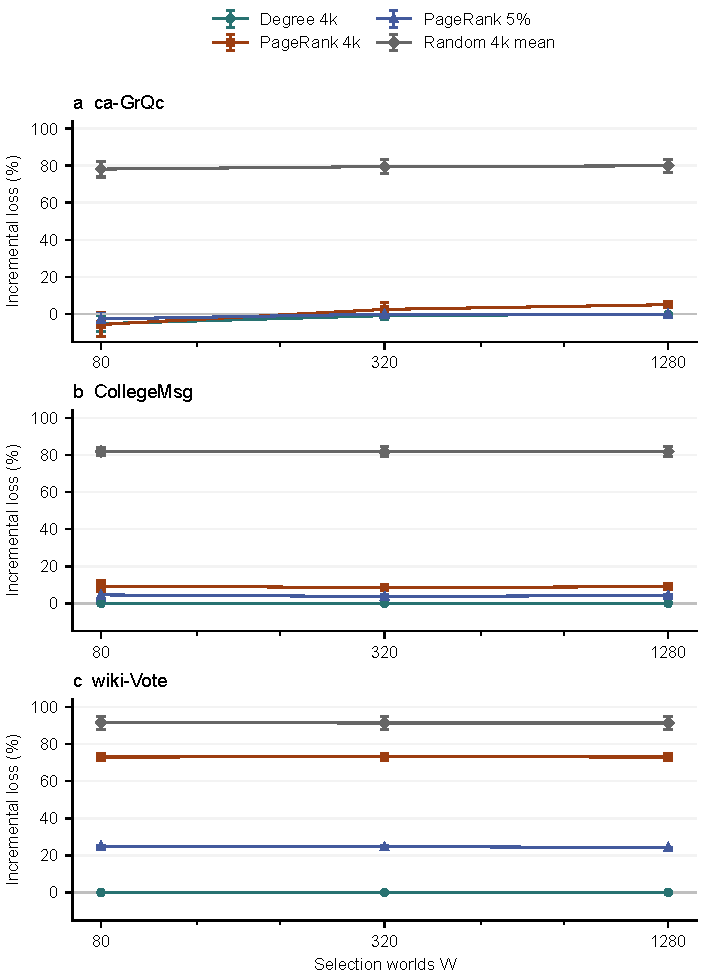
\includegraphics[width=\linewidth]{Fig1.pdf}
\caption{Complete default-tolerance budget comparison. Points are mean incremental
losses over five paths; bars are path standard deviations. Random-pool repeats
are averaged within each path. Negative loss denotes independently evaluated
gain against the finite reference; all graph panels use a common percentage
scale.}\label{fig:matrix}
\end{figure}
\section{Post-hoc PageRank precision control}
The frozen default tolerance is $10^{-6}$, and NetworkX stops on a successive
vector $L_1$ change below $n$ times that value. A candidate-only diagnostic at
$10^{-12}$ changed some pool members on ca-GrQc and wiki-Vote; pools agreed
between $10^{-12}$ and $10^{-14}$. Before inspecting new utility outputs, a
separate protocol froze two PageRank arms on every graph and all five original
$W=1280$ paths. Its 15 conditions and 30 arms are a numerical sensitivity control,
not independent confirmation and not additional paths in the primary tests.

Table~\ref{tab:precision} shows that tightening tolerance changes ca-GrQc's 4k
mean difference from $-0.25082$ to $+0.02608$, replacing all five selected sets.
Its original small loss is therefore not precision-robust. CollegeMsg outcomes
are unchanged. wiki-Vote's 4k loss remains large ($-41.21970$, or 73.96\% of
incremental spread), and its 5\% loss is 24.47\%. This diagnostic qualifies the
ranking interpretation without replacing any original observation or retroactively
redefining the frozen sign-test family. Tightened-solver timing is not substituted
into the default-solver cost curves.
\begin{table}[htbp]
\caption{Post-hoc precision control at $W=1280$, tolerance $10^{-12}$. Difference is versus the frozen full-candidate reference; change is versus the default PageRank implementation. Order compares with default PageRank, not full eligibility. These are the original five paths, not new independent samples.}\label{tab:precision}
\begin{tabular}{llrrrr}
\toprule
Graph & Pool & Difference & Loss (\%) & Change & Order \\
\midrule
ca-GrQc & PageRank-4k & 0.02608 & -0.54 & +0.27690 & 0/5 \\
ca-GrQc & PageRank-5\% & 0.00000 & 0.00 & +0.00000 & 5/5 \\
CollegeMsg & PageRank-4k & -0.90780 & 9.01 & +0.00000 & 5/5 \\
CollegeMsg & PageRank-5\% & -0.43094 & 4.28 & +0.00000 & 5/5 \\
wiki-Vote & PageRank-4k & -41.21970 & 73.96 & -0.52636 & 0/5 \\
wiki-Vote & PageRank-5\% & -13.63982 & 24.47 & -0.10970 & 3/5 \\
\bottomrule
\end{tabular}
\end{table}

\section{Post-hoc precision--budget control}
The initial precision control left a material question open because it covered
only $W=1280$. A new protocol was frozen before new utility outputs were inspected
and added PageRank-4k and PageRank-5\% arms at the tighter tolerance at $W=80,320$ for all three
graphs and five original paths. It contributes 30 conditions and 60 restricted
arms, reusing the frozen full references and disjoint evaluation-world IDs. Together
with the prior tighter-tolerance $W=1280$ layer, this is a 45-condition, 90-arm post-hoc
sensitivity study; it adds no independent paths or primary tests.

Candidate membership agrees between $10^{-12}$ and $10^{-14}$ for every graph/pool size. This checks membership stability at the tested cutoffs, not exact PageRank-vector convergence.
CollegeMsg's tighter- and default-tolerance pools are identical. ca-GrQc changes two of 20
4k candidates (pool Jaccard .818), while wiki-Vote changes one (Jaccard .905).
The lower-budget results show that ca-GrQc's default PageRank-4k direction reversal
disappears with the tighter-tolerance pool: incremental losses are -11.25\%, -2.96\% and
-0.54\% at $W=80,320,1280$. Its selected sets and paired utility magnitude still
change with budget. CollegeMsg retains 9.33\%, 8.52\% and 9.01\% 4k losses at the tighter tolerance;
wiki-Vote retains 74.05\%, 74.05\% and 73.96\%. These are graph-specific,
post-hoc sensitivity findings, not an equivalence, superiority or significance claim.
\begin{table}[htbp]
\caption{Post-hoc PageRank loss across budgets. Each entry is the mean incremental-loss percentage across five original paths at $W=80/320/1280$. Default uses NetworkX tolerance $10^{-6}$; Tighter uses $10^{-12}$, with candidate membership unchanged at $10^{-14}$. Pool Jaccard compares default- and tighter-tolerance candidates. This is a numerical sensitivity analysis, not a new primary test family.}\label{tab:precision-budget}
\begin{tabular}{llrrr}
\toprule
Graph & Pool & Default loss (\%) & Tighter loss (\%) & Pool Jaccard \\
\midrule
ca-GrQc & 4k & -5.61 / 2.53 / 5.07 & -11.25 / -2.96 / -0.54 & 0.818 \\
ca-GrQc & 5\% & -2.62 / 0.00 / 0.00 & -2.62 / 0.00 / 0.00 & 0.977 \\
CollegeMsg & 4k & 9.33 / 8.52 / 9.01 & 9.33 / 8.52 / 9.01 & 1.000 \\
CollegeMsg & 5\% & 4.57 / 3.72 / 4.28 & 4.57 / 3.72 / 4.28 & 1.000 \\
wiki-Vote & 4k & 73.01 / 73.06 / 73.01 & 74.05 / 74.05 / 73.96 & 0.905 \\
wiki-Vote & 5\% & 24.91 / 24.67 / 24.28 & 24.83 / 24.67 / 24.47 & 0.994 \\
\bottomrule
\end{tabular}
\end{table}

\section{Coverage, direction and reference transitions}
The direction illustration in Fig.~\ref{fig:direction-detail} supports a
graph-specific interpretation of wiki-Vote's loss. At $W=1280$, path 1101 gives
the full seed set $\{2565,766,11,457,2688\}$.
The PageRank-4k set is $\{3352,2237,2328,2654,1297\}$.
The same final sets occur on all five paths.
The PageRank pool contains none of the full-reference seeds. Its mean incremental
spread is 15.04268 nodes, compared with 55.73602 for full selection, a paired
difference of $-40.69334$ nodes. These coverage facts are consistent with a
mismatch between incoming importance and outgoing propagation; without a
direction intervention they do not establish causality.
\begin{figure}[htbp]
\centering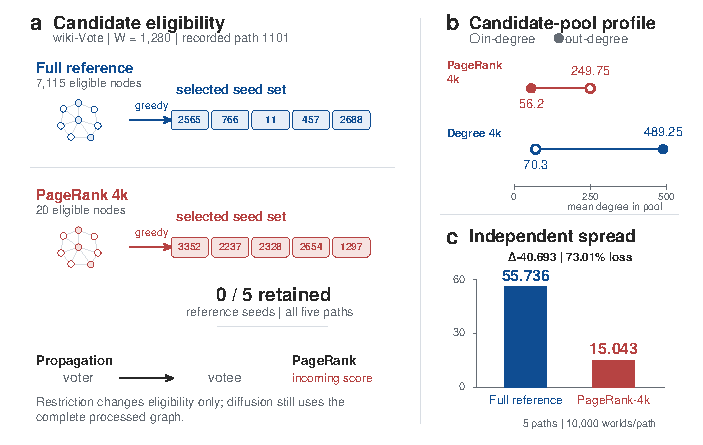
\includegraphics[width=\linewidth]{FigDirectionMechanism.pdf}
\caption{Post-hoc direction and candidate-coverage diagnostic for wiki-Vote.
The illustrated seed sets, stored voter-to-votee orientation and independent
spread values connect candidate eligibility to the measured loss at $W=1280$.
The diagram describes this graph and propagation convention.}\label{fig:direction-detail}
\end{figure}
Table~\ref{tab:transitions} supplies the aggregate reference-transition values
underlying the main-text paired spread plot. Identical final sets have identical
evaluation vectors and hence exactly zero paired differences.
\begin{table}[htbp]
\caption{Full-reference transitions under step coupling. Gain is the paired independent change in total spread; seed counts are constant. The range is across paths, not a confidence interval.}\label{tab:transitions}
\begin{tabular}{llrrr}
\toprule
Graph & Budgets & Set changed & Mean gain & Path range \\
\midrule
ca-GrQc & 80--320 & 5/5 & +0.39616 & +0.1819, +0.6139 \\
ca-GrQc & 320--1280 & 5/5 & +0.12720 & -0.0266, +0.2411 \\
CollegeMsg & 80--320 & 2/5 & +0.09994 & +0.0000, +0.2855 \\
CollegeMsg & 320--1280 & 1/5 & +0.05336 & +0.0000, +0.2668 \\
wiki-Vote & 80--320 & 0/5 & +0.00000 & +0.0000, +0.0000 \\
wiki-Vote & 320--1280 & 0/5 & +0.00000 & +0.0000, +0.0000 \\
\bottomrule
\end{tabular}
\end{table}


\section{Descriptive utility--cost thresholds}
Figure~\ref{fig:loss-cost} retains all frozen loss thresholds. Degree-4k meets
zero point-estimate loss on every highest-budget path. Default PageRank-4k meets
10\% on ca-GrQc and CollegeMsg, but not 20\% on wiki-Vote. The 5\% PageRank
pool meets zero loss on ca-GrQc and 5\% on CollegeMsg, and still fails 20\% on
wiki-Vote. No within-path random-pool mean meets 20\%. These thresholds are
descriptive; no application-specific acceptable loss or noninferiority margin
is inferred. Timing at the tighter tolerance is not substituted into this analysis.
\begin{figure}[htbp]
\centering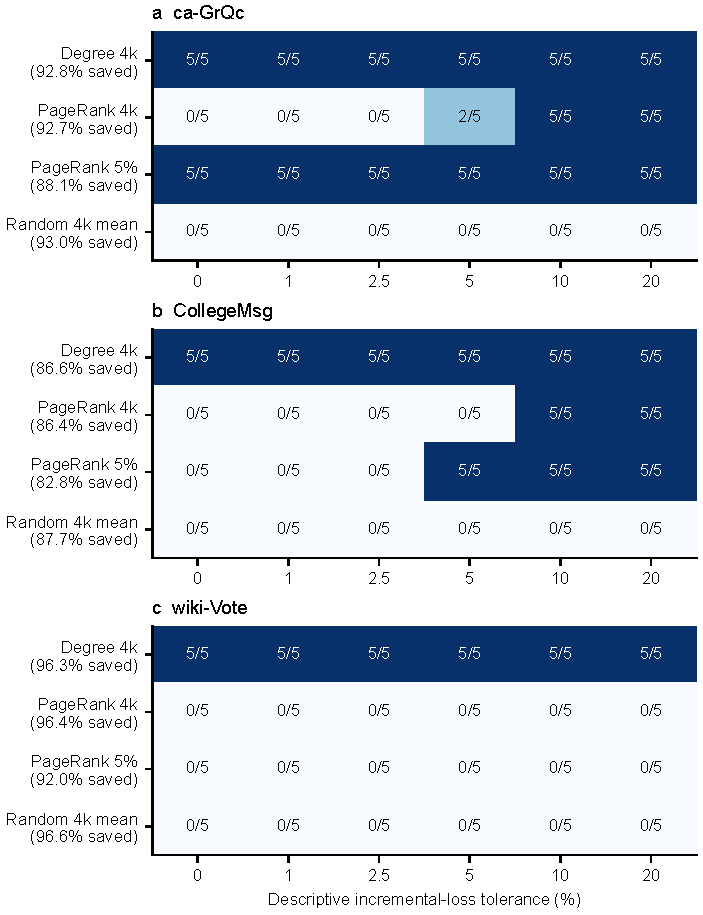
\includegraphics[width=\linewidth]{Fig3.pdf}
\caption{Loss--cost decisions for default tolerance at $W=1280$. Cells count
paths with point-estimate incremental loss at or below the column threshold.
Row labels show mean assembled verification-inclusive savings across all five
paths. Random rows average three pools within each path and use the mean cost
of one random-pool deployment.}\label{fig:loss-cost}
\end{figure}
\section{Coupling control}
Figure~\ref{fig:coupling} shows all preselected W320 control paths for the main
ranking comparisons. Mean PageRank-4k differences under edge coupling are
$-0.16240$, $-0.93417$ and $-40.57597$ on ca-GrQc, CollegeMsg and wiki-Vote.
Degree-4k ordered agreement is 1/3, 3/3 and 3/3, respectively. This control
preserves the prominent PageRank losses while showing that coupling can change
reference reproduction. It does not estimate a general coupling-invariance law.
\begin{figure}[htbp]
\centering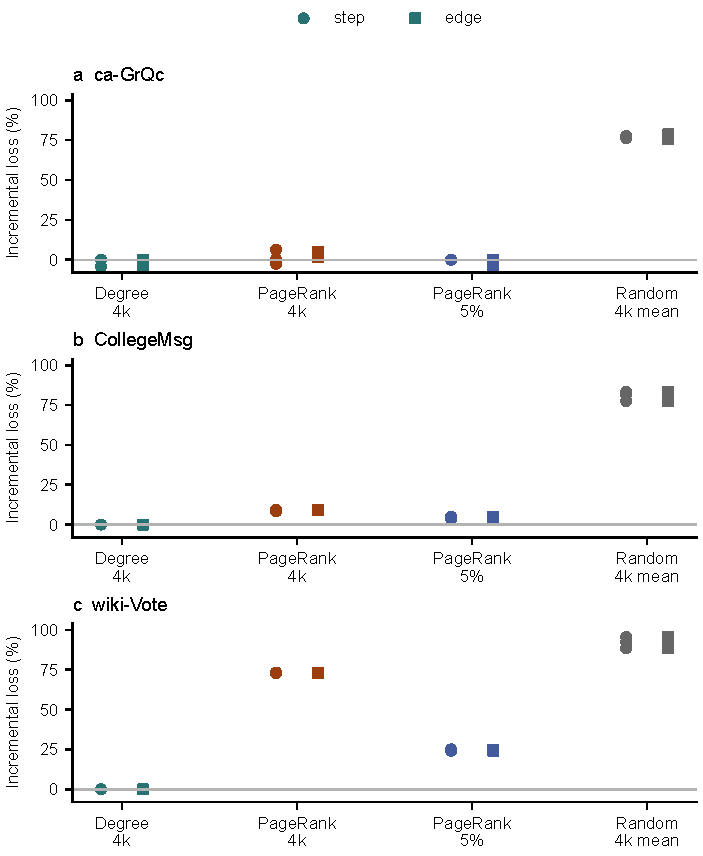
\includegraphics[width=\linewidth]{FigS1.pdf}
\caption{Coupling control at $W=320$. Each symbol is one of three preselected
computational paths, with three random-pool repetitions first averaged within
path. Circles denote step-indexed worlds and squares fixed-edge worlds. Loss is
relative to the full reference using the same coupling. No inferential intervals
are implied by these point displays}\label{fig:coupling}
\end{figure}
\FloatBarrier
\section{Executable reproduction procedure}
\subsection{Inputs, identifiers and numerical environment}
The external package root contains \texttt{config.json}, \texttt{protocol.md},
\texttt{snapshot/}, \texttt{data/source\_manifest.json} and
\texttt{results/main/}. The default study has 54 JSON/NPZ pairs and 468 arms.
The two post-hoc controls remain under \texttt{review-v2/} and
\texttt{review-v3-budget-precision/}; they contain 15 and 30 conditions,
respectively, with two restricted arms per condition. These outputs must not be
merged with the main-study count.

The namespace is \path{computing-external-validation-20261015-v1}.
For dataset $d$, path $r$, family $f$ and world index $i$, the exact UTF-8 key is
\begin{center}\texttt{namespace|dataset|path|family|i}\end{center}
using decimal integers without padding.
The world ID is the first eight SHA-256 bytes, interpreted as an unsigned
big-endian integer and masked to 63 bits. Families are \texttt{selection} and
\texttt{evaluation}; indices start at zero. World-to-edge draws use the frozen
unsigned-64-bit mixing function in \texttt{legacy\_engine.py}, with a 53-bit
uniform output. In the step coupling the step index enters this function; the
fixed-edge coupling uses step zero throughout. Replacing this mapping with a
different pseudorandom generator would not reproduce the archived paths.

Random-pool keys are \texttt{namespace|pool|dataset|path|repeat}, with repetition
indices 0, 1 and 2. Their first eight SHA-256 bytes, without the 63-bit mask,
seed NumPy's \texttt{default\_rng}; for the external $k=5$ study, the first 20 entries of a node permutation
form the pool. Greedy evaluation sorts these candidate indices before scanning
them. Lexicographic node indexing makes the first integer-score maximizer the
specified tie winner. PageRank uses the graph insertion order generated by
the frozen reader, so reproductions retain that order as well as its tolerance.

Core dependencies are pinned in \texttt{requirements.txt}; the checked environment
is Python 3.13.0 on Windows. Pillow 12.3.0 is additionally used for decoded-pixel
comparison. TeX Live 2026 and Poppler support manuscript compilation and rendering,
but are unnecessary for the propagation calculation. The reproduction wrapper
sets OpenMP, OpenBLAS, MKL and Numba thread limits to one before numerical imports.
Its environment record reports the actual installed versions for each run.

\subsection{Commands and acceptance criteria}
The retained external reproduction guide, \path{EXTERNAL_REPRODUCE_INHERITED.md},
gives PowerShell commands for an isolated environment, input acquisition and
the two replay modes. The current \texttt{REPRODUCE.md} separately describes
regeneration of historical summaries without simulation. For external replay, run
\texttt{src/reproduce.py} from the revised package with explicit
\texttt{--base} and a fresh \texttt{--output}. The base is the external package
root; the output must not exist. The script checks original source, raw-file,
processed-graph and main-result hashes before computation. It preserves the
source tree and builds a working copy for legacy analysis scripts whose output
paths are fixed relative to their own locations.

The \texttt{representative} mode reruns path 1101 for all three graphs at
$W=80$ with step coupling and $W=320$ with fixed-edge coupling. It also reruns
PageRank with the tighter tolerance at $W=80,1280$ on that path, covering both precision protocols.
The \texttt{all} mode reruns all 54 main conditions and all 45 post-hoc
precision conditions. The \texttt{none} mode checks saved results and regenerates
analysis without rerunning seed selection or propagation; it still reconstructs
graphs and candidate pools and checks world identifiers. Raw inputs are required in all modes
because graph hashes and direction diagnostics are reconstructed.

A replay passes only if selected IDs, every integer candidate score and every
one of the 10,000 evaluation counts match their archived counterparts exactly.
The analysis stage independently recomputes paired differences and Monte Carlo
standard errors from saved arrays, applies the frozen aggregation and test rules,
and regenerates the default and precision plots. CSV values are compared at
absolute and relative tolerance $10^{-12}$; decoded PNG pixels must be identical.
The machine-readable report records counts, checks and any failure. Fresh wall
times, process memory, PDF metadata and SVG metadata are not equality targets.
Cross-platform font rendering may fail the pixel check even when numerical
tables agree; such a difference requires inspection rather than silent acceptance.

The archived reproduction record documents representative-mode execution and
complete external analysis regeneration, not a rerun of every historical
experiment or every external condition. Historical summary verification reads
saved arrays without replaying selection or propagation.
Historical evidence retains its separate frozen package and reproduction guide.
The saved setup-timing table is an input to the assembled cost analysis; regenerating
that analysis does not remeasure all setup costs on the current machine.

\clearpage
\section{Historical sensitivity evidence}\label{sec:historical-evidence}
\subsection{Coverage, provenance and statistical units}
Table~\ref{tab:hist-coverage} separates the evidence layers and the five batches
within the historical extension. Contact graphs retain the first 65\% of complete
timestamp groups. Undirected contacts become reciprocal propagation arcs;
repeated events are collapsed for topology and counted for historical weighted
degree. Propagation probability remains uniform, independently of these counts.
The initial study's protocol and 42 condition records establish its coverage;
its outputs are not pooled with the later extension or the external study.
\begin{longtable}{p{.23\linewidth}p{.51\linewidth}p{.14\linewidth}}
\caption{Evidence layers and experiment coverage. A condition fixes graph, path, $k,p,h,W$ and coupling; an arm changes eligibility. Paths are computational replicates. Counts are not independent network sample sizes.}\label{tab:hist-coverage}\\
\toprule Batch / graphs & Selection design and evaluation & Conditions / arms\\\midrule\endfirsthead
\multicolumn{3}{l}{\tablename~\thetable{} (continued)}\\\toprule
Batch / graphs & Selection design and evaluation & Conditions / arms\\\midrule\endhead\bottomrule\endfoot
Initial study / C4, C3 & C4: $k=5$; C3: $k=20$. $p=.01$, $h=3$, $W=20,80,320$, step; two paths (301--302); $M=2000$. Initial weighted-pool/reference comparisons. & 42 / 168\\
Historical budget / C4 & $k=5$, $p=.01$, $h=3$, $W=20,80,320,1280,5120$, step; ten paths (1001--1010); $M=10{,}000$. Reference-budget sensitivity. & 200 / 1800\\
Historical parameters / C4 & $k=5$, $W=320$, step; $(p,h)=(.005,3),(.05,3),(.01,1),(.01,5)$; ten paths; $M=10{,}000$. Local parameter changes. Default $(.01,3)$ reuses 40 budget conditions. & 160 / 1440\\
Historical coupling / C4 & $k=5$, $p=.01$, $h=3$, $W=320,1280$, fixed edge; ten paths; $M=10{,}000$. Coupling-specific comparisons and budget transitions. & 80 / 720\\
Historical larger seeds / C3 & $k=20$, $p=.01$, $h=3$, $W=320,1280$, step; ten paths; $M=10{,}000$. Seed-budget and coverage control. & 60 / 540\\
Historical synthetic / S2 & $k=5$, $p=.01$, $h=3$, $W=80,320$, step; five paths (1001--1005) per fixed instance; $M=10{,}000$. Topology controls. & 20 / 180\\
External primary / E3 & $k=5$, $p=.01$, $h=3$, $W=80,320,1280$, step; five paths (1101--1105); $M=10{,}000$. External transfer, budget and pool coverage. & 45 / 390\\
External coupling / E3 & $k=5$, $p=.01$, $h=3$, $W=320$, fixed edge; three paths (1101--1103); $M=10{,}000$. Coupling control. & 9 / 78\\
Post-hoc precision / E3 & PageRank-4k/5\% at the tighter tolerance, $W=80,320,1280$, step; other settings, five paths and $M=10{,}000$ reused from primary study. Existing full references reused. Numerical sensitivity, not new independent replication. & 45 / 90\\
\end{longtable}
\noindent C4: invs2013 ($n=91$), invs2015 (212), kenya2012 (75), sfhh2009 (402).
C3 excludes sfhh2009. S2: one BA and one SBM instance, each $n=2000$.
E3: CollegeMsg (1438), ca-GrQc (5241), wiki-Vote (7115).
Historical extension totals are $200+160+80+60+20=520$ conditions and 4680 arms.
Its nine arms are full selection, Weighted-2k/4k/8k, Degree-4k, PageRank-4k and three random-4k pools.
The external matrix totals 54 conditions and 468 arms. Resource-only preflight is outside all outcome totals.


The 520-condition extension locally froze its protocol after the initial study
and resource preflight. It is not a public preregistration. All nine arms use
the complete propagation graph and differ only in seed eligibility, with a
common lexical tie rule. Candidate sizes are capped at the number of vertices.
The namespace is \texttt{computing-extension-20261015-v1}; selection and evaluation
families have separate hash keys. Selection budgets use nested world prefixes.
Historical PageRank uses the frozen default numerical settings; these controls
are distinct from the external post-hoc tolerance study.

The historical summary audit covers all 520 stored JSON/NPZ pairs. Their 1,040 file
hashes match the result manifest, and the historical engine hash matches the
external package's legacy engine. Means, paired differences and conditional
Monte Carlo standard errors are recomputed from all 4,680 saved arm vectors,
each containing 10,000 counts. Seven path-level method summaries result after
averaging the three random pools within each path. The 3,640 path rows,
378 group rows (reported means and sample standard deviations) and 240 adjacent
budget transitions agree with the saved analyses. This verifies file integrity
and the specified numerical summaries, not every aspect of the study design.
These checks reaggregate saved results; they do not replay selection or propagation.

For each path, $\Delta$ is restricted minus full mean spread. The reported loss
is $-100\Delta/(\widehat\sigma_{\rm full}-k)$, averaged across paths after forming
each path's ratio; all denominators are positive. A negative loss denotes a
point-estimate gain. Table SDs describe variation across paths, not confidence
intervals for a population of networks. Conditional Monte Carlo standard errors
come from the paired per-world differences for fixed selected sets. Random-pool
vectors are averaged before calculating their conditional errors; the pools do
not triple the path count. The same path used at multiple settings is a repeated
measurement. No new hypothesis tests are introduced here, and no historical
paths are pooled with the five external paths.

\subsection{Local propagation-parameter changes}
Table~\ref{tab:hist-parameters} and Fig.~\ref{fig:hist-parameters} include all
four preselected nondefault settings and the reused default setting at $W=320$.
They vary probability or horizon around the default, rather than forming a full
factorial design. Over the 160 nondefault conditions, Degree-4k and PageRank-4k
reproduce 117 and 132 ordered full-reference trajectories. Each has one negative
paired spread difference; positive differences occur in 42 and 27 conditions,
respectively. Weighted-4k reproduces none of these trajectories and has 117
negative and 43 positive differences. These counts summarize the retained
conditions; they are not independent Bernoulli trials.

The weighted-ranking discrepancy varies with graph and setting. At $(p,h)=(.05,3)$,
its mean differences are $-0.51309$, $-1.52602$, $+0.07939$ and $-4.98321$ nodes
for invs2013, invs2015, kenya2012 and sfhh2009, respectively. The corresponding
mean incremental losses are 4.12\%, 2.37\%, $-0.89$\% and 4.09\%.
Thus neither a single sign nor the absolute difference alone summarizes the
parameter control. Complete results for Weighted-2k/8k and the within-path
random mean remain in the accompanying all-method CSVs.
\begin{figure}[p]
\centering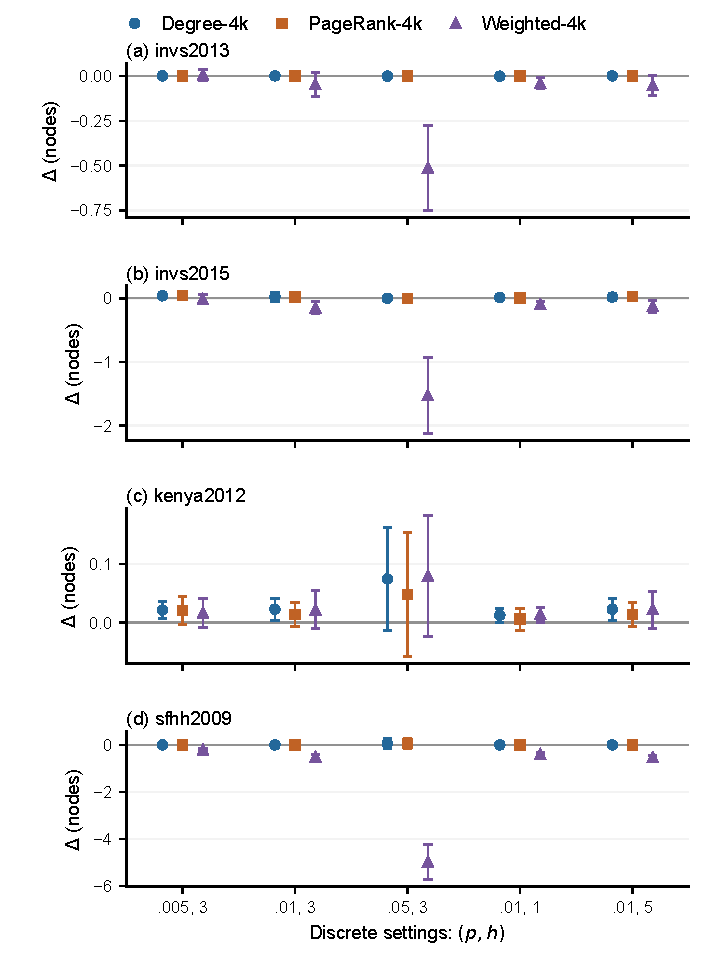
\includegraphics[width=\linewidth]{HistoryParameters.pdf}
\caption{Historical parameter sensitivity for three 4k rankings, with $k=5$,
$W=320$ and step coupling. Each panel is one contact graph; each point is the mean
paired spread difference over ten paths, and bars are one path standard deviation.
Settings are discrete, not a continuous sweep. Vertical scales differ between
panels. Positive differences favor the restricted set. The default $(.01,3)$
reuses the budget scan. These are path-variation bars, not conditional Monte Carlo
intervals or uncertainty across networks.}\label{fig:hist-parameters}
\end{figure}
\FloatBarrier
\begin{longtable}{llrrrrr}
\caption{Historical propagation-parameter sensitivity at $k=5$, $W=320$, step coupling. D, P and W denote Degree-4k, PageRank-4k and Weighted-4k. $\Delta$ is restricted minus full spread (nodes); SD is across paths; loss is the mean pathwise incremental loss (\%), negative when restriction gains. Match counts refer to the entire ordered sequence. Coverage is the fraction of eligible vertices (\%). The default $(.01,3)$ rows reuse the budget scan; they are not additional conditions.}\label{tab:hist-parameters}\\
\toprule
$(p,h)$ & Rank & $\overline\Delta$ & SD & Loss & Match & Cov. \\
\midrule
\endfirsthead
\multicolumn{7}{l}{\tablename~\thetable{} (continued)}\\
\toprule
$(p,h)$ & Rank & $\overline\Delta$ & SD & Loss & Match & Cov. \\
\midrule
\endhead
\bottomrule
\endfoot
\multicolumn{7}{l}{\textit{invs2013}}\\*
0.005, 3 & D & +0.0016 & 0.0068 & -0.25 & 8/10 & 21.98\\*
0.005, 3 & P & +0.0016 & 0.0068 & -0.25 & 8/10 & 21.98\\*
0.005, 3 & W & +0.0044 & 0.0301 & -0.76 & 0/10 & 21.98\\*
0.01, 1 & D & +0.0000 & 0.0000 & +0.00 & 10/10 & 21.98\\*
0.01, 1 & P & +0.0000 & 0.0000 & +0.00 & 10/10 & 21.98\\*
0.01, 1 & W & -0.0386 & 0.0309 & +2.85 & 0/10 & 21.98\\*
0.01, 3 & D & +0.0014 & 0.0046 & -0.10 & 9/10 & 21.98\\*
0.01, 3 & P & +0.0014 & 0.0046 & -0.10 & 9/10 & 21.98\\*
0.01, 3 & W & -0.0467 & 0.0664 & +2.93 & 0/10 & 21.98\\*
0.01, 5 & D & +0.0014 & 0.0045 & -0.09 & 9/10 & 21.98\\*
0.01, 5 & P & +0.0014 & 0.0045 & -0.09 & 9/10 & 21.98\\*
0.01, 5 & W & -0.0507 & 0.0553 & +3.22 & 0/10 & 21.98\\*
0.05, 3 & D & +0.0000 & 0.0000 & +0.00 & 10/10 & 21.98\\*
0.05, 3 & P & +0.0000 & 0.0000 & +0.00 & 10/10 & 21.98\\*
0.05, 3 & W & -0.5131 & 0.2380 & +4.12 & 0/10 & 21.98\\
\multicolumn{7}{l}{\textit{invs2015}}\\*
0.005, 3 & D & +0.0385 & 0.0413 & -2.25 & 5/10 & 9.43\\*
0.005, 3 & P & +0.0392 & 0.0459 & -2.31 & 5/10 & 9.43\\*
0.005, 3 & W & -0.0186 & 0.0709 & +0.93 & 0/10 & 9.43\\*
0.01, 1 & D & +0.0124 & 0.0391 & -0.43 & 9/10 & 9.43\\*
0.01, 1 & P & +0.0063 & 0.0198 & -0.21 & 9/10 & 9.43\\*
0.01, 1 & W & -0.0986 & 0.0486 & +3.23 & 0/10 & 9.43\\*
0.01, 3 & D & +0.0200 & 0.0632 & -0.47 & 9/10 & 9.43\\*
0.01, 3 & P & +0.0200 & 0.0632 & -0.47 & 9/10 & 9.43\\*
0.01, 3 & W & -0.1500 & 0.0940 & +3.35 & 0/10 & 9.43\\*
0.01, 5 & D & +0.0186 & 0.0588 & -0.42 & 9/10 & 9.43\\*
0.01, 5 & P & +0.0242 & 0.0515 & -0.53 & 8/10 & 9.43\\*
0.01, 5 & W & -0.1327 & 0.0929 & +2.89 & 0/10 & 9.43\\*
0.05, 3 & D & +0.0000 & 0.0000 & +0.00 & 10/10 & 9.43\\*
0.05, 3 & P & +0.0000 & 0.0000 & +0.00 & 10/10 & 9.43\\*
0.05, 3 & W & -1.5260 & 0.5980 & +2.37 & 0/10 & 9.43\\
\multicolumn{7}{l}{\textit{kenya2012}}\\*
0.005, 3 & D & +0.0214 & 0.0142 & -4.45 & 0/10 & 26.67\\*
0.005, 3 & P & +0.0210 & 0.0238 & -4.43 & 3/10 & 26.67\\*
0.005, 3 & W & +0.0165 & 0.0246 & -3.47 & 0/10 & 26.67\\*
0.01, 1 & D & +0.0125 & 0.0117 & -1.33 & 4/10 & 26.67\\*
0.01, 1 & P & +0.0059 & 0.0188 & -0.67 & 9/10 & 26.67\\*
0.01, 1 & W & +0.0138 & 0.0127 & -1.47 & 0/10 & 26.67\\*
0.01, 3 & D & +0.0228 & 0.0185 & -2.10 & 3/10 & 26.67\\*
0.01, 3 & P & +0.0135 & 0.0205 & -1.24 & 6/10 & 26.67\\*
0.01, 3 & W & +0.0218 & 0.0323 & -2.01 & 0/10 & 26.67\\*
0.01, 5 & D & +0.0228 & 0.0184 & -2.09 & 3/10 & 26.67\\*
0.01, 5 & P & +0.0136 & 0.0207 & -1.25 & 6/10 & 26.67\\*
0.01, 5 & W & +0.0220 & 0.0317 & -2.03 & 0/10 & 26.67\\*
0.05, 3 & D & +0.0745 & 0.0878 & -0.83 & 1/10 & 26.67\\*
0.05, 3 & P & +0.0481 & 0.1057 & -0.54 & 7/10 & 26.67\\*
0.05, 3 & W & +0.0794 & 0.1031 & -0.89 & 0/10 & 26.67\\
\multicolumn{7}{l}{\textit{sfhh2009}}\\*
0.005, 3 & D & +0.0000 & 0.0000 & +0.00 & 10/10 & 4.98\\*
0.005, 3 & P & +0.0041 & 0.0130 & -0.12 & 9/10 & 4.98\\*
0.005, 3 & W & -0.2285 & 0.0591 & +6.32 & 0/10 & 4.98\\*
0.01, 1 & D & +0.0000 & 0.0000 & +0.00 & 10/10 & 4.98\\*
0.01, 1 & P & +0.0000 & 0.0000 & +0.00 & 10/10 & 4.98\\*
0.01, 1 & W & -0.4063 & 0.0622 & +6.68 & 0/10 & 4.98\\*
0.01, 3 & D & +0.0000 & 0.0000 & +0.00 & 10/10 & 4.98\\*
0.01, 3 & P & +0.0000 & 0.0000 & +0.00 & 10/10 & 4.98\\*
0.01, 3 & W & -0.5211 & 0.1040 & +5.93 & 0/10 & 4.98\\*
0.01, 5 & D & +0.0000 & 0.0000 & +0.00 & 10/10 & 4.98\\*
0.01, 5 & P & +0.0000 & 0.0000 & +0.00 & 10/10 & 4.98\\*
0.01, 5 & W & -0.5421 & 0.1085 & +5.90 & 0/10 & 4.98\\*
0.05, 3 & D & +0.0650 & 0.2055 & -0.05 & 9/10 & 4.98\\*
0.05, 3 & P & +0.0650 & 0.2055 & -0.05 & 9/10 & 4.98\\*
0.05, 3 & W & -4.9832 & 0.7338 & +4.09 & 0/10 & 4.98\\
\end{longtable}


\subsection{Fixed-edge control and reference-budget transitions}
Table~\ref{tab:hist-coupling} compares each ranking with the full reference under
the same sampling scheme. At $W=1280$, Degree-4k matches 38/40 trajectories and
PageRank-4k matches 40/40 under both schemes. Weighted-4k matches 7/40 under step
coupling and 5/40 under fixed-edge coupling. At $W=320$, Degree-4k matches 31/40
under either scheme, while PageRank-4k matches 34/40 and 35/40, respectively.
These agreement patterns persist on the historical contact graphs, although
individual paths and the weighted method's utility gaps differ. Evaluation
counts from step and fixed-edge sampling are not subtracted element by element;
all reported method differences use their own scheme-specific reference.
\begin{longtable}{llrrrrr}
\caption{Historical coupling controls at $k=5$, $p=.01$, $h=3$. Each row uses its own coupling-specific full reference. D, P and W denote Degree-4k, PageRank-4k and Weighted-4k. $\Delta$ is restricted minus full spread (nodes); SD is across paths; loss is the mean pathwise incremental loss (\%), negative when restriction gains. Match counts refer to the entire ordered sequence. Coverage is the fraction of eligible vertices (\%).}\label{tab:hist-coupling}\\
\toprule
Coupling, $W$ & Rank & $\overline\Delta$ & SD & Loss & Match & Cov. \\
\midrule
\endfirsthead
\multicolumn{7}{l}{\tablename~\thetable{} (continued)}\\
\toprule
Coupling, $W$ & Rank & $\overline\Delta$ & SD & Loss & Match & Cov. \\
\midrule
\endhead
\bottomrule
\endfoot
\multicolumn{7}{l}{\textit{invs2013}}\\*
edge, 320 & D & -0.0022 & 0.0069 & +0.15 & 9/10 & 21.98\\*
edge, 320 & P & -0.0022 & 0.0069 & +0.15 & 9/10 & 21.98\\*
edge, 320 & W & -0.0515 & 0.0338 & +3.36 & 0/10 & 21.98\\*
step, 320 & D & +0.0014 & 0.0046 & -0.10 & 9/10 & 21.98\\*
step, 320 & P & +0.0014 & 0.0046 & -0.10 & 9/10 & 21.98\\*
step, 320 & W & -0.0467 & 0.0664 & +2.93 & 0/10 & 21.98\\*
edge, 1280 & D & +0.0000 & 0.0000 & +0.00 & 10/10 & 21.98\\*
edge, 1280 & P & +0.0000 & 0.0000 & +0.00 & 10/10 & 21.98\\*
edge, 1280 & W & -0.0610 & 0.0136 & +3.90 & 0/10 & 21.98\\*
step, 1280 & D & +0.0000 & 0.0000 & +0.00 & 10/10 & 21.98\\*
step, 1280 & P & +0.0000 & 0.0000 & +0.00 & 10/10 & 21.98\\*
step, 1280 & W & -0.0652 & 0.0254 & +4.15 & 0/10 & 21.98\\
\multicolumn{7}{l}{\textit{invs2015}}\\*
edge, 320 & D & +0.0225 & 0.0496 & -0.52 & 8/10 & 9.43\\*
edge, 320 & P & +0.0143 & 0.0452 & -0.33 & 9/10 & 9.43\\*
edge, 320 & W & -0.1677 & 0.1232 & +3.73 & 0/10 & 9.43\\*
step, 320 & D & +0.0200 & 0.0632 & -0.47 & 9/10 & 9.43\\*
step, 320 & P & +0.0200 & 0.0632 & -0.47 & 9/10 & 9.43\\*
step, 320 & W & -0.1500 & 0.0940 & +3.35 & 0/10 & 9.43\\*
edge, 1280 & D & +0.0000 & 0.0000 & +0.00 & 10/10 & 9.43\\*
edge, 1280 & P & +0.0000 & 0.0000 & +0.00 & 10/10 & 9.43\\*
edge, 1280 & W & -0.2057 & 0.0554 & +4.52 & 0/10 & 9.43\\*
step, 1280 & D & +0.0000 & 0.0000 & +0.00 & 10/10 & 9.43\\*
step, 1280 & P & +0.0000 & 0.0000 & +0.00 & 10/10 & 9.43\\*
step, 1280 & W & -0.2049 & 0.0522 & +4.52 & 0/10 & 9.43\\
\multicolumn{7}{l}{\textit{kenya2012}}\\*
edge, 320 & D & +0.0202 & 0.0212 & -1.86 & 4/10 & 26.67\\*
edge, 320 & P & +0.0156 & 0.0254 & -1.46 & 7/10 & 26.67\\*
edge, 320 & W & +0.0067 & 0.0292 & -0.65 & 1/10 & 26.67\\*
step, 320 & D & +0.0228 & 0.0185 & -2.10 & 3/10 & 26.67\\*
step, 320 & P & +0.0135 & 0.0205 & -1.24 & 6/10 & 26.67\\*
step, 320 & W & +0.0218 & 0.0323 & -2.01 & 0/10 & 26.67\\*
edge, 1280 & D & +0.0026 & 0.0059 & -0.23 & 8/10 & 26.67\\*
edge, 1280 & P & +0.0000 & 0.0000 & +0.00 & 10/10 & 26.67\\*
edge, 1280 & W & +0.0015 & 0.0145 & -0.14 & 5/10 & 26.67\\*
step, 1280 & D & +0.0039 & 0.0092 & -0.35 & 8/10 & 26.67\\*
step, 1280 & P & +0.0000 & 0.0000 & +0.00 & 10/10 & 26.67\\*
step, 1280 & W & +0.0010 & 0.0124 & -0.10 & 7/10 & 26.67\\
\multicolumn{7}{l}{\textit{sfhh2009}}\\*
edge, 320 & D & +0.0000 & 0.0000 & +0.00 & 10/10 & 4.98\\*
edge, 320 & P & +0.0000 & 0.0000 & +0.00 & 10/10 & 4.98\\*
edge, 320 & W & -0.5416 & 0.0813 & +6.15 & 0/10 & 4.98\\*
step, 320 & D & +0.0000 & 0.0000 & +0.00 & 10/10 & 4.98\\*
step, 320 & P & +0.0000 & 0.0000 & +0.00 & 10/10 & 4.98\\*
step, 320 & W & -0.5211 & 0.1040 & +5.93 & 0/10 & 4.98\\*
edge, 1280 & D & +0.0000 & 0.0000 & +0.00 & 10/10 & 4.98\\*
edge, 1280 & P & +0.0000 & 0.0000 & +0.00 & 10/10 & 4.98\\*
edge, 1280 & W & -0.6158 & 0.0212 & +6.94 & 0/10 & 4.98\\*
step, 1280 & D & +0.0000 & 0.0000 & +0.00 & 10/10 & 4.98\\*
step, 1280 & P & +0.0000 & 0.0000 & +0.00 & 10/10 & 4.98\\*
step, 1280 & W & -0.6295 & 0.0329 & +7.08 & 0/10 & 4.98\\
\end{longtable}


The reference-transition analysis pairs only budgets within the same
graph, path and coupling, and verifies that their saved evaluation-world hashes agree.
Under step coupling, $W=1280\to5120$ changes 16/40 final sets, with a descriptive
mean gain of 0.01111 nodes and range $[-0.0383,0.1180]$. Under fixed-edge coupling,
$W=320\to1280$ changes 29/40 sets, with mean gain 0.061845 nodes and range
$[-0.0110,0.2572]$. Table~\ref{tab:hist-transitions} retains the network-specific
results, and Fig.~\ref{fig:hist-edge-transitions} shows every fixed-edge path.
The two intervals in $W$ differ: their averages cannot be interpreted as a
controlled estimate of a coupling effect. Both distinguish reference-set changes
from their spread consequences; neither establishes optimality with respect to expected spread or
convergence. In particular, these historical controls do not test whether the
external ca-GrQc result at the tighter PageRank tolerance persists under fixed-edge sampling.
\begin{table}[htbp]
\caption{Full-reference budget transitions within each graph, path and coupling. Changes count final sets; spread differences are high minus low budget (nodes), with SD across ten paths.}\label{tab:hist-transitions}
\centering\begin{tabular}{lrrrrr}
\toprule
Graph & Changed & Mean & SD & Min & Max\\
\midrule
\multicolumn{6}{l}{\textit{Step: $1280\to5120$}}\\
invs2013 & 1/10 & +0.00481 & 0.01521 & +0.0000 & +0.0481\\
invs2015 & 5/10 & +0.02462 & 0.04981 & -0.0383 & +0.1180\\
kenya2012 & 10/10 & +0.01501 & 0.01427 & -0.0105 & +0.0336\\
sfhh2009 & 0/10 & +0.00000 & 0.00000 & +0.0000 & +0.0000\\
\multicolumn{6}{l}{\textit{Fixed edge: $320\to1280$}}\\
invs2013 & 7/10 & +0.04391 & 0.04082 & +0.0000 & +0.1050\\
invs2015 & 6/10 & +0.09937 & 0.11329 & +0.0000 & +0.2572\\
kenya2012 & 10/10 & +0.02906 & 0.02221 & -0.0110 & +0.0557\\
sfhh2009 & 6/10 & +0.07504 & 0.06776 & +0.0000 & +0.1770\\
\bottomrule
\end{tabular}
\end{table}

\begin{figure}[p]
\centering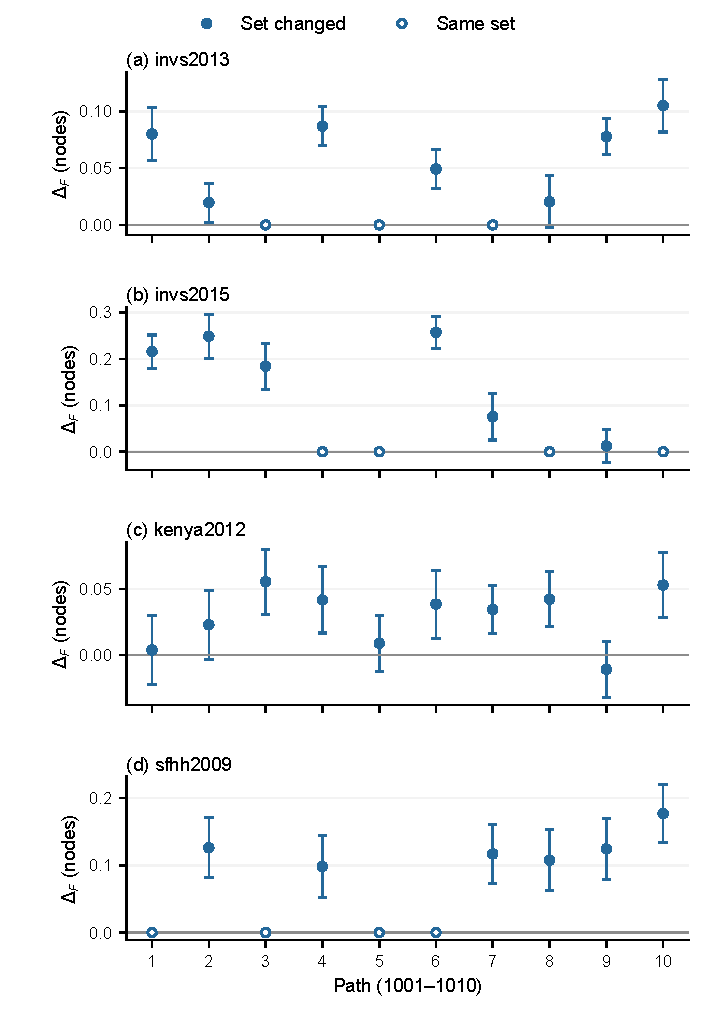
\includegraphics[width=\linewidth]{HistoryEdgeTransitions.pdf}
\caption{Historical fixed-edge full-reference changes from $W=320$ to 1280.
Each point is one computational path's paired high-minus-low spread difference;
filled points indicate a changed final set. Bars are unadjusted pointwise
$\Delta_F\pm1.96\,\mathrm{SE}_{\rm MC}$ intervals from 10,000 saved paired worlds,
conditional on the selected sets. They do not represent path or network
uncertainty. Panel-specific scales are used. All 40 paths are retained, including
negative and zero differences.}\label{fig:hist-edge-transitions}
\end{figure}
\FloatBarrier

\subsection{Larger seed budget and fixed synthetic instances}
Table~\ref{tab:hist-secondary} reports the secondary controls separately. At
$k=20$, a nominal 4k pool contains all 75 kenya2012 vertices. Its exact agreement
is therefore a full-candidate consistency check, not evidence of useful pruning.
The invs2013 pool retains 80/91 vertices (87.91\%), and invs2015 retains 80/212
(37.74\%); these coverage levels differ substantially from the external 20-node
pools. No sfhh2009 condition with $k=20$ was executed in this extension.

The synthetic controls use one BA instance with attachment parameter 3 and one
SBM instance with four 500-vertex blocks, within-block probability .012 and
between-block probability .0005; graph-generation seed is 20261015. Both have
2,000 vertices and reciprocal arcs. Their weights derive from topology rather
than observed contact events, so Weighted-4k is not independent historical-event
evidence. At $W=320$, all three displayed rankings reproduce all five BA
trajectories. On the fixed SBM instance, Degree-4k and PageRank-4k reproduce 1/5
and 0/5, with mean spread differences of $+0.04052$ and $+0.03756$ nodes. These
are finite-reference comparisons on two fixed graphs; five paths per graph do
not constitute five independently generated networks.
\begin{longtable}{llrrrrr}
\caption{Secondary historical controls: $k=20$ for the three contact graphs and $k=5$ for the two fixed synthetic instances; $p=.01$, $h=3$, step coupling. D, P and W denote Degree-4k, PageRank-4k and Weighted-4k. $\Delta$ is restricted minus full spread (nodes); SD is across paths; loss is the mean pathwise incremental loss (\%), negative when restriction gains. Match counts refer to the entire ordered sequence. Coverage is the fraction of eligible vertices (\%). Synthetic W denotes topology-derived weights, not observed event frequency.}\label{tab:hist-secondary}\\
\toprule
$W$ & Rank & $\overline\Delta$ & SD & Loss & Match & Cov. \\
\midrule
\endfirsthead
\multicolumn{7}{l}{\tablename~\thetable{} (continued)}\\
\toprule
$W$ & Rank & $\overline\Delta$ & SD & Loss & Match & Cov. \\
\midrule
\endhead
\bottomrule
\endfoot
\multicolumn{7}{l}{\textit{invs2013}}\\*
320 & D & +0.0000 & 0.0000 & +0.00 & 10/10 & 87.91\\*
320 & P & +0.0000 & 0.0000 & +0.00 & 10/10 & 87.91\\*
320 & W & -0.0006 & 0.0019 & +0.02 & 9/10 & 87.91\\*
1280 & D & +0.0000 & 0.0000 & +0.00 & 10/10 & 87.91\\*
1280 & P & +0.0000 & 0.0000 & +0.00 & 10/10 & 87.91\\*
1280 & W & +0.0000 & 0.0000 & +0.00 & 10/10 & 87.91\\
\multicolumn{7}{l}{\textit{invs2015}}\\*
320 & D & +0.0268 & 0.0462 & -0.22 & 5/10 & 37.74\\*
320 & P & +0.0265 & 0.0464 & -0.22 & 6/10 & 37.74\\*
320 & W & -0.0066 & 0.1290 & +0.05 & 0/10 & 37.74\\*
1280 & D & +0.0078 & 0.0247 & -0.06 & 9/10 & 37.74\\*
1280 & P & +0.0000 & 0.0000 & +0.00 & 10/10 & 37.74\\*
1280 & W & -0.1162 & 0.0565 & +0.92 & 0/10 & 37.74\\
\multicolumn{7}{l}{\textit{kenya2012}}\\*
320 & D & +0.0000 & 0.0000 & +0.00 & 10/10 & 100.00\\*
320 & P & +0.0000 & 0.0000 & +0.00 & 10/10 & 100.00\\*
320 & W & +0.0000 & 0.0000 & +0.00 & 10/10 & 100.00\\*
1280 & D & +0.0000 & 0.0000 & +0.00 & 10/10 & 100.00\\*
1280 & P & +0.0000 & 0.0000 & +0.00 & 10/10 & 100.00\\*
1280 & W & +0.0000 & 0.0000 & +0.00 & 10/10 & 100.00\\
\pagebreak[4]
\multicolumn{7}{l}{\textit{synthetic\_ba2000}}\\*
80 & D & +0.0000 & 0.0000 & +0.00 & 5/5 & 1.00\\*
80 & P & +0.0000 & 0.0000 & +0.00 & 5/5 & 1.00\\*
80 & W & +0.0000 & 0.0000 & +0.00 & 5/5 & 1.00\\*
320 & D & +0.0000 & 0.0000 & +0.00 & 5/5 & 1.00\\*
320 & P & +0.0000 & 0.0000 & +0.00 & 5/5 & 1.00\\*
320 & W & +0.0000 & 0.0000 & +0.00 & 5/5 & 1.00\\
\multicolumn{7}{l}{\textit{synthetic\_sbm2000}}\\*
80 & D & +0.1326 & 0.0542 & -21.80 & 0/5 & 1.00\\*
80 & P & +0.1307 & 0.0537 & -21.46 & 0/5 & 1.00\\*
80 & W & +0.1326 & 0.0542 & -21.80 & 0/5 & 1.00\\*
320 & D & +0.0405 & 0.0386 & -5.71 & 1/5 & 1.00\\*
320 & P & +0.0376 & 0.0241 & -5.23 & 0/5 & 1.00\\*
320 & W & +0.0405 & 0.0386 & -5.71 & 1/5 & 1.00\\
\end{longtable}


\subsection{Traceability and scope}
The historical tables and figures are generated from saved results and metadata
by \texttt{src/integrate\_historical.py}. All-method CSVs retain arm metrics,
within-path random means, group summaries, candidate coverage and reference
transitions; figure-source CSVs contain every displayed value.
\texttt{REPRODUCE.md} records the aggregation commands and checks.

Historical controls describe sensitivity on the tested contact networks;
parameter coverage on the external networks remains narrow. Their descriptive
summaries neither add independent external paths nor change the post-hoc
identity of the PageRank control. The cost comparisons retain the exhaustive
full-candidate reference used in the experiments.

\section{File map and availability}
The full reproducibility materials comprise frozen sources and protocols,
manifests, external and historical results, per-path analyses and manuscript
assets. Historical aggregation scripts, source CSVs and verification records
accompany the manuscript; frozen experiment packages remain separate. Raw
third-party inputs are obtained through the guarded download instructions and
are not redistributed. No public archive URL is asserted.
\end{document}
